\documentclass{IEEEtran}
\usepackage[pdftex]{graphicx}
\usepackage{cite}
\newcommand{\HRule}{\rule{\linewidth}{0.5mm}}
\usepackage{color}
\usepackage{listings}
\definecolor{mygreen}{rgb}{0,0.6,0}
\definecolor{mygray}{rgb}{0.9,0.9,0.9}
\definecolor{mymauve}{rgb}{0.58,0,0.52}
\lstset{
  backgroundcolor=\color{mygray},     % choose the background color; you must add \usepackage{color} or \usepackage{xcolor}
  basicstyle=\tiny\ttfamily,  % the size of the fonts that are used for the code
  breakatwhitespace=false,            % sets if automatic breaks should only happen at whitespace
  breaklines=true,                    % sets automatic line breaking
  captionpos=b,                       % sets the caption-position to bottom
  commentstyle=\color{mygreen},       % comment style
  deletekeywords={...},               % if you want to delete keywords from the given language
  escapeinside={\%*}{*)},             % if you want to add LaTeX within your code
  extendedchars=true,                 % lets you use non-ASCII characters; for 8-bits encodings only, does not work with UTF-8
  frame=single,                       % adds a frame around the code
  keepspaces=true,                    % keeps spaces in text, useful for keeping indentation of code (possibly needs columns=flexible)
  keywordstyle=\color{blue},          % keyword style
  language=Verilog,                   % the language of the code
  morekeywords={*,...},               % if you want to add more keywords to the set
  numbers=left,                       % where to put the line-numbers; possible values are (none, left, right)
  numbersep=5pt,                      % how far the line-numbers are from the code
  numberstyle=\tiny\color{mygray},    % the style that is used for the line-numbers
  rulecolor=\color{black},            % if not set, the frame-color may be changed on line-breaks within not-black text (e.g. comments (green here))
  showspaces=false,                   % show spaces everywhere adding particular underscores; it overrides 'showstringspaces'
  showstringspaces=false,             % underline spaces within strings only
  showtabs=false,                     % show tabs within strings adding particular underscores
  stepnumber=2,                       % the step between two line-numbers. If it's 1, each line will be numbered
  stringstyle=\color{mymauve},        % string literal style
  tabsize=1,                          % sets default tabsize to 2 spaces
  %title=\lstname                      % show the filename of files included with \lstinputlisting; also try caption instead of title
}

\begin{document}
\begin{titlepage}
\begin{center}

% Upper part of the page. The '~' is needed because \\
% only works if a paragraph has started.
%\includegraphics[width=0.15\textwidth]{./logo}~\\[1cm]

\textsc{\LARGE CSU Sacramento}\\[1.5cm]

\textsc{\Large EEE 188: Digital Control Systems}\\[0.5cm]

% Title
\HRule \\[0.4cm]
{ \huge \bfseries Two Axis Gimbal v0.2\\[0.4cm] }

\HRule \\[1.5cm]

% Author and supervisor
\begin{minipage}{0.4\textwidth}
\begin{flushleft} \large
\emph{Author:}\\
Curtis \textsc{Muntz}\\
David \textsc{Larribas}\\
Michael \textsc{Frith}
\end{flushleft}
\end{minipage}
\begin{minipage}{0.4\textwidth}
\begin{flushright} \large
\emph{Instructor:} \\
Dr. \textsc{Belkhouche}
\end{flushright}
\end{minipage}

\vfill

% Bottom of the page
{\large \today}

\end{center}
\end{titlepage}
\vfill

\begin{abstract}
A 2-axis gimbal controlled by an Arduino Uno microcontroller. The angle is determined by an IMU sensor which provides accelerometer and gyroscope data. The microcontroller processes this data using a complementary filter. A Taylor series approximation is used to determine the angle accurately up to $30^\circ$. This system uses the feedback from the sensors in an attempt to stabilize itself to the angles read.
\end{abstract}

\section{Intro}
We are tasked with building a project that takes a sensor, a microcontroller, and an actuator to create a control system. We decided to build a 2-axis gimbal, a device that keeps a camera's attitude nominally consistent in the chosen axes regardless of its mounted system. If a gimbal is attached to a multi rotor helicopter, it will keep the camera level independent of the pitch and roll of the airframe.

\section{Progress Made Last Semester}
As a review of last semester's progress, we implemented a gimbal system in order to maintain a constant attitude of a camera, mounted on a moving platform, through the control of two servo motors. We utilized the accelerometer and gyroscope from the MPU-6050 6-DOF sensor to write a sensor fusion algorithm to obtain precise angular measurements. Camera orientation was controlled using proportional feedback control. The final prototype is shown in Figure \ref{physicalPIC}. The goal of this semester was to update our control scheme from proportional control into a PID algorithm.

\begin{figure}[ht!]
    \centering
    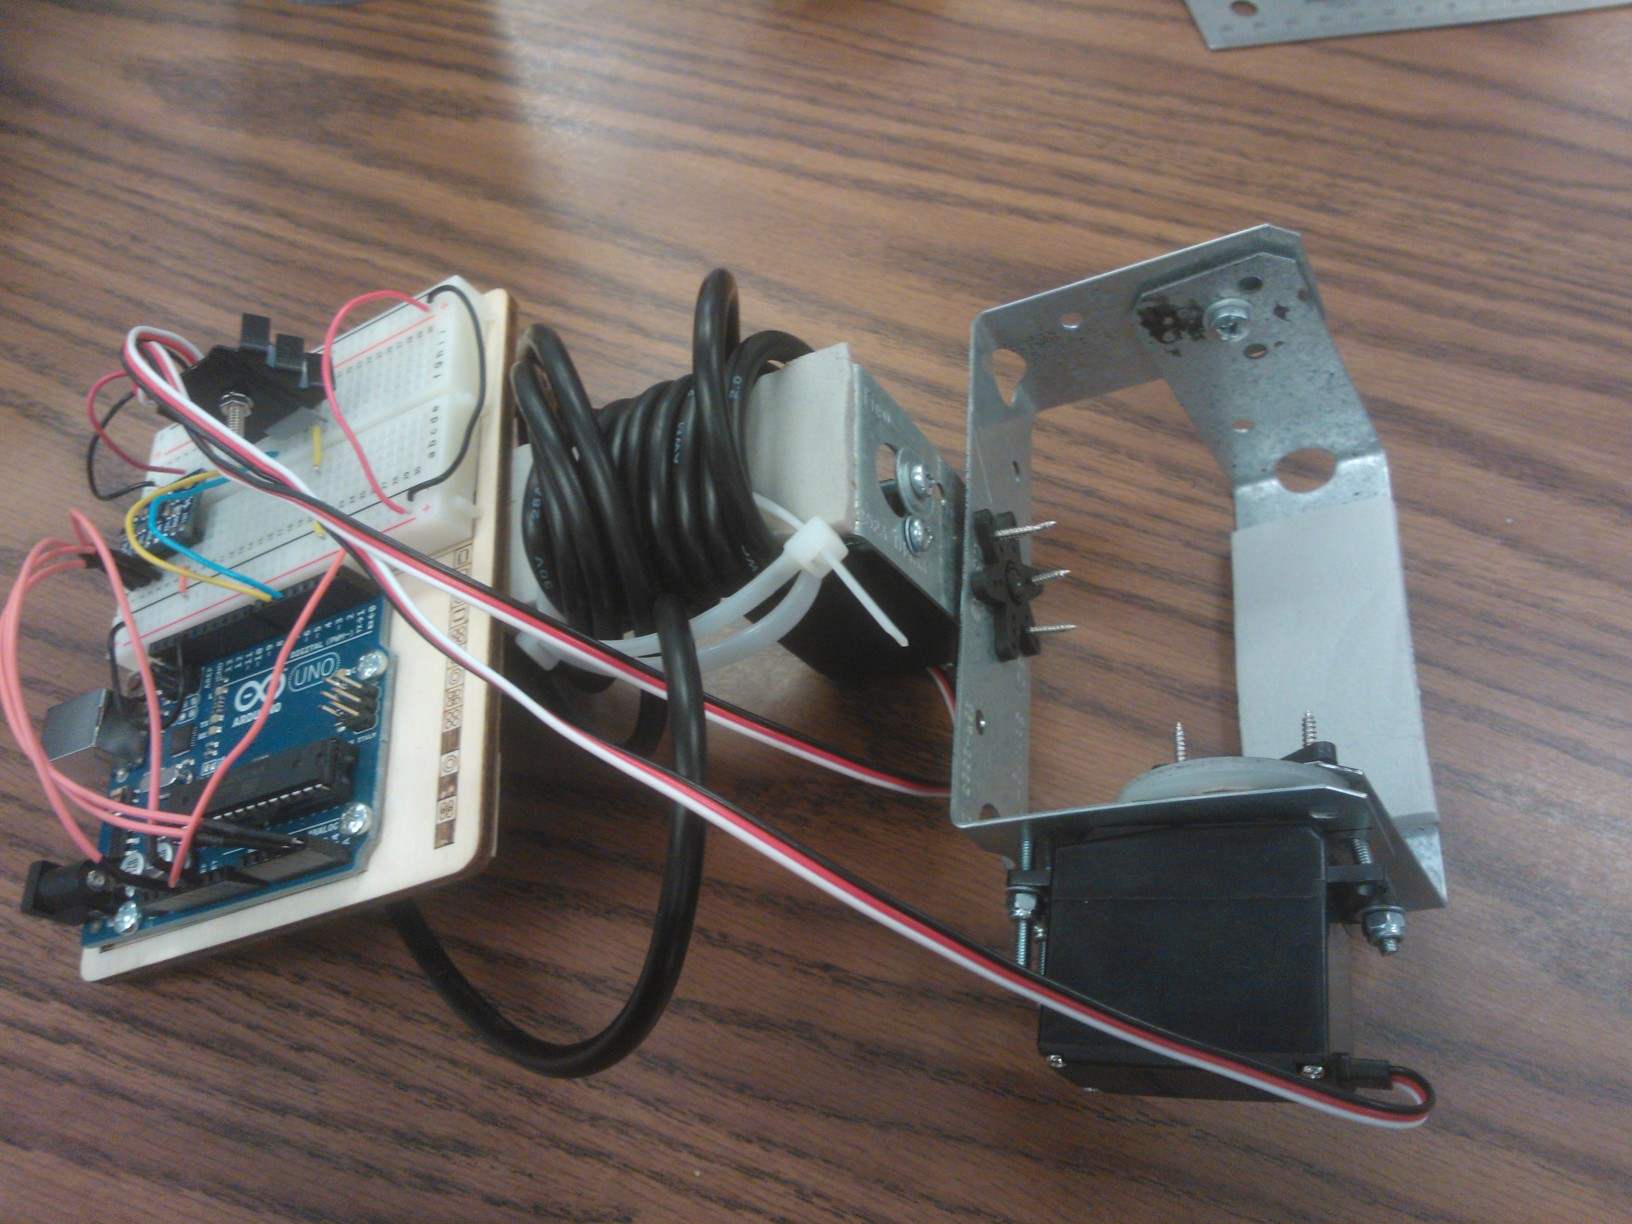
\includegraphics[width=0.4\textwidth]{../physical}
    \caption{\emph{Physical Layout}}
    \label{physicalPIC}
\end{figure}


\section{Updating Drivers}
After discovering important data sheet information provided by the manufacturer of the MEMS chips, the interface between the Arduino microcontroller and the I2C sensors was written from scratch. Last semester, we borrowed example code provided by Jeff Rowberg \cite{rowberg} in order to interface with the digital sensor. This semester, we took the time in order to write our own I2C driver. Furthermore, the data acquisition was refined, as the actual parameters of the sensor were found, instead of using parameters estimated through experimentation.

\section{PID Algorithm and the Brick Wall}
In order to update the 

But the system only really works if the values $Kp = -1$, $Ki = 0$, and $Kd = 0$. If we have any sort of values assigned to the $Ki$ or $Kd$ terms, the system goes beyond its range of usability. This is because we do not have control over the speed of the servo motors.

\section{Conclusions}

\bibliographystyle{apacite}
\bibliography{bussingpaper}

\end{document}